
\section{Release Notes}

The purpose of the ESMF v1.0 release was to provide a first look at the ESMF
Application Programming Interface (API), and to demonstrate the viability 
of the ESMF architecture and implementation.  For that release we focused 
on implementing major architectural features and basic functionality.  The 
performance characteristics and memory requirements of the software 
are unlikely to resemble those in later releases.

We are relying on Earth system modelers to provide us with the feedback 
necessary to realize this goal.  Section \ref{sec:Support} of this document 
includes instructions on submitting comments on ESMF v1.0 to our 
development team.

We are providing roughly monthly {\it internal releases} which are snapshots
of the source code tree and must be compiled before being used.  While these
releases are tested, there will be known bugs in them which are documented,
along with advances in functionality, on the {\tt Internal Releases} web page
located at the ESMF web site {\tt www.esmf.ucar.edu}.

Our next major release, ESMF v2.0, will occur in April 2004.  At that time, 
the {\it ESMF Reference Manual} will cover a broader range of functionality
and the interfaces and documentation will be more polished and consistent.  
We anticipate, but have 
not scheduled, other public releases and patches between now and ESMF v2.0.  
Our focus during this year will be on developing an easy to use, 
production-quality product.  


\section{What is the Earth System Modeling Framework?}

The Earth System Modeling Framework (ESMF) is a structured collection of 
software building blocks that can be used or customized to develop 
Earth system model components, and assemble them into applications.  
The simplest view of the ESMF is that it consists of an
{\it infrastructure} of utilities and data structures for creating 
model components, and a {\it superstructure} for coupling them.  
User code sits between these two layers, making calls to the infrastructure
libraries beneath it and being scheduled and synchronized by the 
superstructure above it.  The configuration resembles a sandwich, as
shown in Figure~\ref{fig:TheESMFwich}.

The ESMF architecture is scalable, flexible paradigm for building highly 
complex climate, weather, and related applications from components such
as atmospheric models, land models, and data assimilation systems.  The 
ESMF is not a single master application into which all components must fit; 
rather it is a way of developing components so that they can be used 
in many different user-written applications.  Model components that adopt 
ESMF are usable in different contexts without code modification, and may be
incorporated into other ESMF-based modeling systems within the Earth 
science community.  In addition to high-level organization, ESMF provides 
a set of robust, portable, performance optimized libraries for regridding, 
data transfers, I/O, time management, and other common modeling functions.  
ESMF users may choose to extensively rewrite their codes to take advantage 
of the ESMF infrastructure, or they may decide to simply wrap user-written 
components in ESMF interfaces in order to adopt the ESMF architecture and 
utilize framework coupling services.

\section{The ESMF Reference Manual for Fortran90}

This {\it ESMF Reference Manual} is a listing of ESMF standard interfaces
for Fortran90.  Interfaces are grouped by class.  A class is an 
object-oriented software design construct that embodies a specific 
concept like a physical field.  (For more on object-oriented
design, how we have implemented object-oriented design in Fortran, and 
how it is used to organize 
ESMF, please see the \htmladdnormallink{{\it ESMF Architecture Document}}
{http://www.esmf.ucar.edu/esmf_docs/ESMF_archdoc}.

The {\it Reference Manual} is divided into two main parts.  The 
first part is a description 
of the classes in the ESMF superstructure, and the second part is a 
description of classes in the ESMF infrastructure.  The major classes
in the ESMF superstructure are Components, which typically represent
large pieces of functionality such as models, model couplers, and 
dynamics and physics packages; and States, which are the data structures
used to store the fields and other data Components require or can 
make available.  There are both data structures and utilities in the ESMF 
infrastructure; classes include but are not limited to Fields, 
collections of Fields (Bundles), Arrays, and utilities for communication,
decomposition, time management, and application configuration.

For a broad overview of how the ESMF software works, see the 
\htmladdnormallink{{\it ESMF User's Guide}}{http://www.esmf.ucar.edu/esmf_docs/ESMF_usrdoc}.  This 

\begin{center}
\begin{figure}
\caption{Schematic of ESMF ``sandwich'' architecture. In this design the framework consists of two parts. An upper level
{\bf Superstructure} layer and a lower-level {\bf Infrastructure} layer. User code is sandwiched between these two layers.}
\label{fig:TheESMFwich}
\scalebox{1.0}{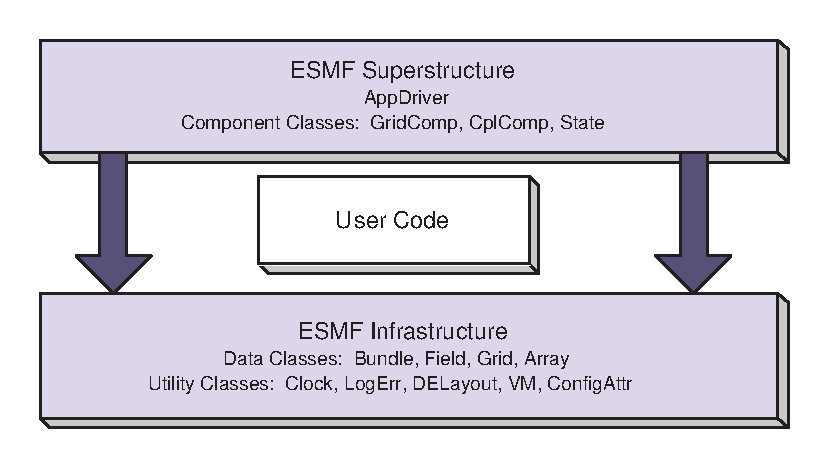
\includegraphics{ESMF_sandwich.eps}}
\end{figure}
\end{center}













